\chapter{Software Process}



\section{Software Process}
A software process is a sequence of activities that leads to the production of a software product.

\textbf{Generic activities in all software processes are:}
(1) Specification (2) Development (3) Validation and (4) Evolution

\textbf{General issues that affect software:}
(1) Heterogeneity, (2) Business and social change, (3) Security and trust, and (4) Scale

\section{Software Process Model}
A software process model is a simplified description of a software process that presents one view of that process. Process models may include activities that are part of the software process, software products and the roles of people involved in software engineering.

\subsection{Process Perspectives}

\begin{enumerate}[itemsep=1ex]
   \item \textbf{Workflow perspective} - sequence of activities, UML Sequence Diagrams
   \item \textbf{Data-flow perspective} - information flow, DFD's
   \item \textbf{Role/action perspective} - who does what. Gantt Charts
\end{enumerate}

\subsubsection*{General models or paradigms of software development:}
$(\text{1})$ The waterfall approach, 
$(\text{2})$ Iterative development, and 
$(\text{3})$ Component-based software engineering (CBSE)


\subsection{Key Types of Software Process Models}

\begin{tabularx}{\textwidth}{|l|X|X|}\hline
   \thl{Factors} & \thl{Prototype Model} & \thl{Incremental Model} \\\hline
   
   \thl{Definition} &
   Develops a working prototype to gather user feedback and refine requirements. &
   Develops the system in small increments, each adding functionality.
   \\\hline

   \thl{Requirement} &
   Not clearly understood or are unstable. &
   Requirements are known up-front and can evolve.\\\hline

   \thl{Risk Handling} &
   Reduces risk by validating requirements early. &
   Reduces risk by delivering smaller, manageable portions of the system. \\\hline

   \thl{User involvement} &
   Customer tested each prototype and gives feedback. &
   Customer tested each prototype and gives feedback. \\\hline

   \thl{Cost} &
   Reduced maintenance cost  &
   Can be high due to frequent changes. \\\hline
\end{tabularx}


\pagebreak
\section{Agile Methodology}
\textbf{Agile model} is a combination of \textbf{iterative} and \textbf{incremental} process models with focus on \orange{process adaptability and customer satisfaction} by \orange{rapid delivery} of working software product. Agile Methods break the product into \textbf{small incremental builds}. These builds are provided in iterations. At the end of the iteration a working product is displayed to the customer and important stakeholders.

\subsection{Core values of Agile Manifesto}

\begin{itemize}[parsep=1ex]
   \item \textbf{Individuals and interactions} over processes and tools.
   \item \textbf{Working software} over comprehensive documentation.
   \item \textbf{Customer collaboration} over contract negotiation.
   \item \textbf{Responding to change} over following a plan.
\end{itemize}

\section{Agile Framework}
\begin{tabularx}{\textwidth}{|l|X|X|}\hline
   \thl{Factors} &
   \thl{Scrum} &
   \thl{Xtreme Programming(XP)}\\\hline

   \thl{Definition} 
   & An iterative Agile framework focused on time-boxed sprints and self-organizing teams.
   & An Agile methodology emphasizing technical excellence, frequent releases, and continuous feedback. \\\hline

   \thl{Iteration Length}
   & 2-4 weeks (Sprints).
   & 1-2 weeks (Shorter cycles). \\\hline
   
   \thl{Focus}
   & Focuses on the process and self-organization.
   & Focuses on the technical aspects of software \, engineering, coding and testing.
   \\\hline

   \thl{Benefit}
   & Helps teams work together.
   & Helps developers to produce a working software model in very short iterations.
   \\\hline

   \thl{Changes in Requirements}
   & Doesn't allow changes while already working on a sprint.
   & Allow changes within its iteration.
   \\\hline

   \thl{Phases}
   & Planning, Design, Coding and Testing.
   & Product backlogs, Sprints, Scrum meeting, and Demos.
   \\\hline
   
   \thl{Team Structure}
   & Product Owner defines backlog,
   Scrum Master prioritizes backlog, Cross-functional Developers Team select and implement sprint backlogs.
   & Developers and customers work closely; customers define user stories, developers implement \& test continuously.
   \\\hline
   
   \thl{Meeting}
   & Sprint Planning Meeting, Sprint Review Meeting, Sprint Retrospective
   & Daily stand-ups, Pair Programming discussions, Continuous feedback. (Optional)
   \\\hline

   \thl{Testing}
   & Testing happens within the sprint.
   & Test-Driven Development is a core practice. \\\hline
     
   \thl{Suitability}
   & Best for larger teams managing complex projects.
   & Best for small, highly collaborative teams focused on quality.
   \\\hline

   \thl{Phase diagram}
   & \centering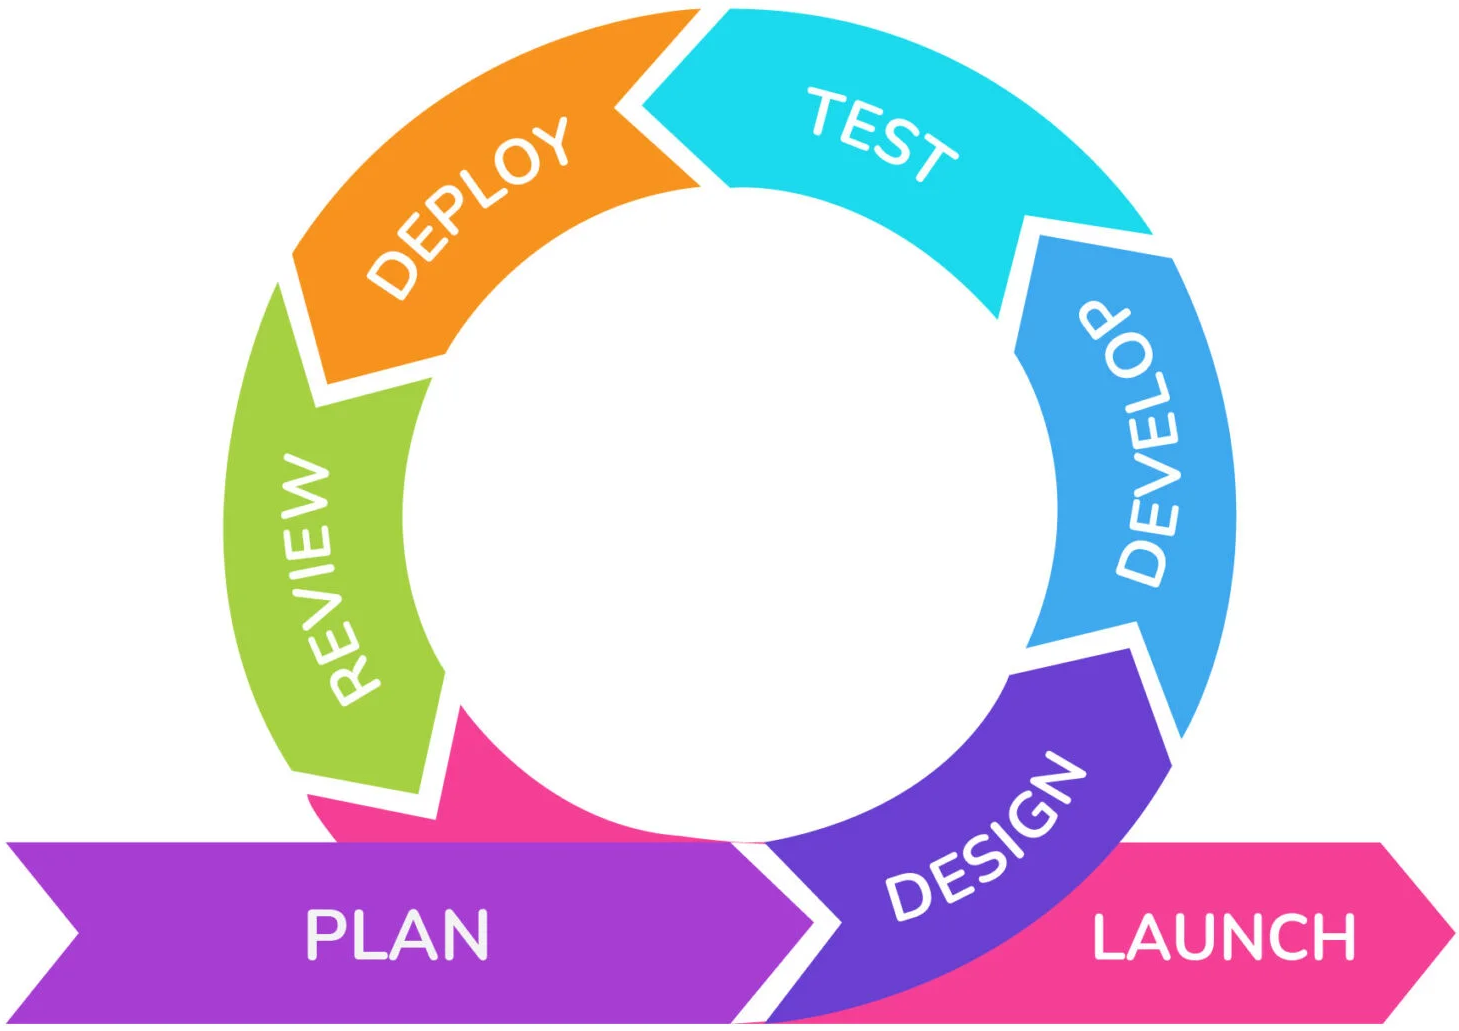
\includegraphics[width=5cm]{figures/agile.png}
   & 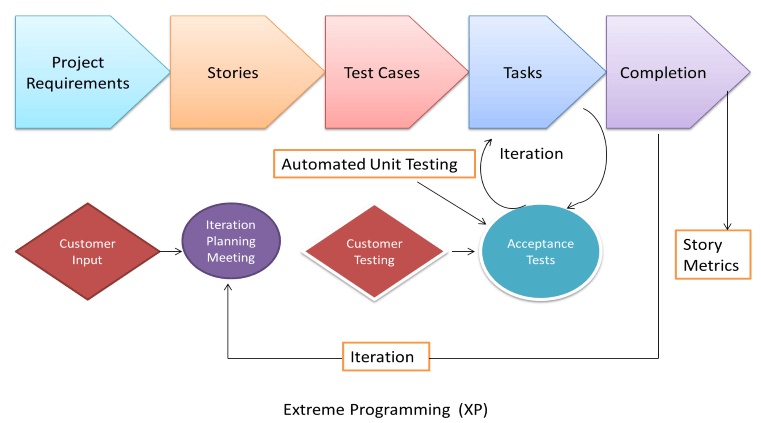
\includegraphics[width=6.5cm]{figures/XP.png}
   \\\hline
\end{tabularx}